\documentclass[10pt]{beamer}

\usepackage{polyglossia}
\usepackage{csquotes}
\usepackage{fontspec}
\usepackage{microtype}
\usepackage{color}
\usepackage{url}
\usepackage[backend=biber,style=iso-authoryear,sortlocale=cs_CZ,autolang=other,bibencoding=UTF8]{biblatex}
\usepackage{booktabs}
\usepackage{hyperref}
\usepackage{amsfonts}
\usepackage{amsthm}
\usepackage{amsmath}

\setdefaultlanguage{czech}
\setotherlanguage{english}
\setmainfont{TeX Gyre Termes}
\usetheme{Boadilla}
\usecolortheme{crane}
\setbeamertemplate{section in toc}[ball unnumbered]
\setbeamertemplate{bibliography item}{}
\addbibresource{zotero.bib}

\hypersetup{
	pdfencoding=auto,
	unicode=true,
	citecolor=green,
	filecolor=blue,
	linkcolor=red,
	urlcolor=blue
}

\makeatletter
\newcommand*{\currentSection}{\@currentlabelname}
\makeatother

\title[Hluboké neuronové sítě pro problémy s hierarchií]
{
	Hluboké neuronové sítě pro problémy s hierarchií
}

\titlegraphic
{
	
\includegraphics[width=0.2\columnwidth]{images/fjfi.png}
}

\author[Marek Dědič]
{
	Marek~Dědič\inst{1} \\
	Školitel:~Ing.~Tomáš~Pevný,~Ph.D.\inst{2}\inst{3}
}

\institute[FJFI ČVUT v Praze]
{
	\inst{1} ČVUT v Praze, Fakulta jaderná a fyzikálně inženýrská, Matematická informatika \and
	\inst{2} Cisco Systems Inc., Karlovo náměstí 10, Praha 2 \and
	\inst{3} ČVUT v Praze, Fakulta elektrotechnická, Katedra počítačů
}

\AtBeginSection[]{
	\begin{frame}{\currentSection}
		\tableofcontents[currentsection]
	\end{frame}
}

\begin{document}

\begin{frame}
	\titlepage
\end{frame}

\begin{frame}{Obsah}
	\tableofcontents
\end{frame}

% Body

\section{Motivace}

\begin{frame}{Motivace - o zpětné propagaci}
	\centering
	\textit{\enquote{But is this what the brain actually does? Alas, the back-prop nets are unrealistic in almost every respect}}\footnote{\cite{crick_recent_1989}}
\end{frame}

\section{Target propagation}

\begin{frame}{Dataset}
	\centering
	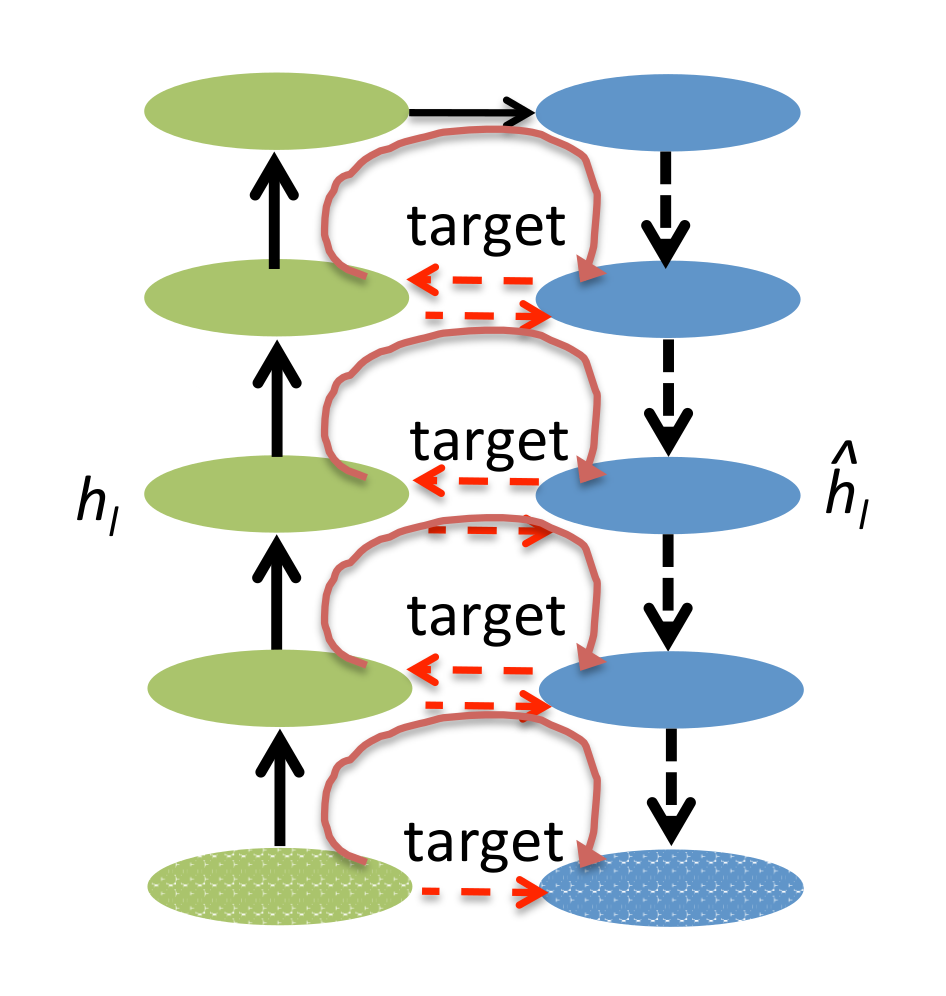
\includegraphics[width=0.55\pagewidth]{images/1407-7906.png}\footnote{\cite{bengio_how_2014}}
\end{frame}

\section{Výsledky}

\begin{frame}{Dataset}
	\centering
	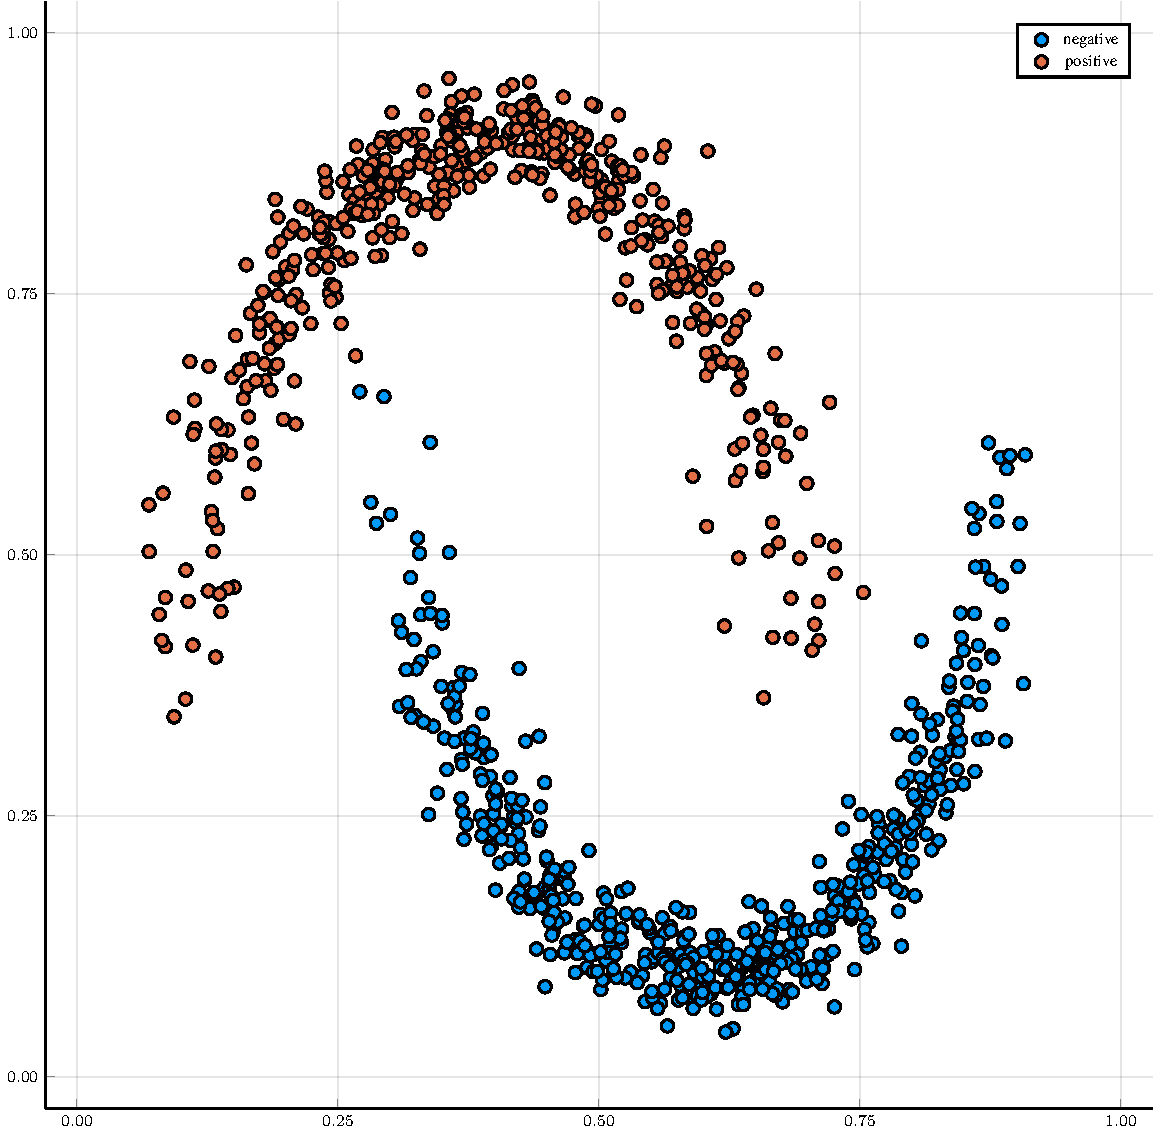
\includegraphics[width=0.6\pagewidth]{images/two-moon/two-moon.pdf}
\end{frame}

\begin{frame}{Zpětná propagace}
	\centering
	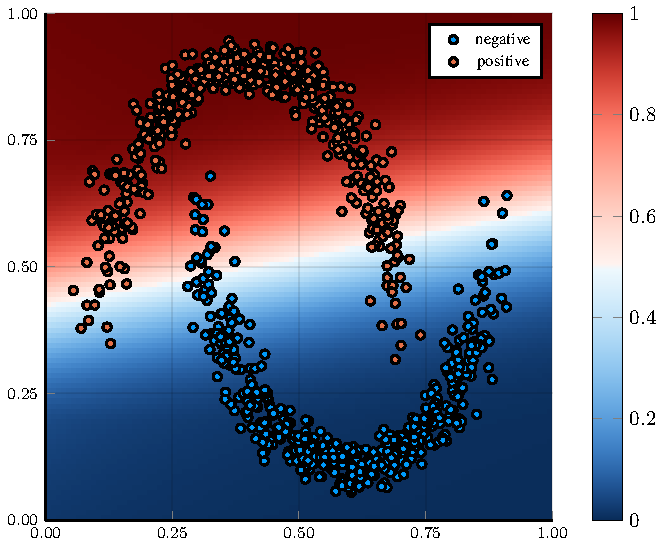
\includegraphics[width=0.6\pagewidth]{images/backprop-heatmap/backprop.pdf}
\end{frame}

\begin{frame}{Target propagation}
	\centering
	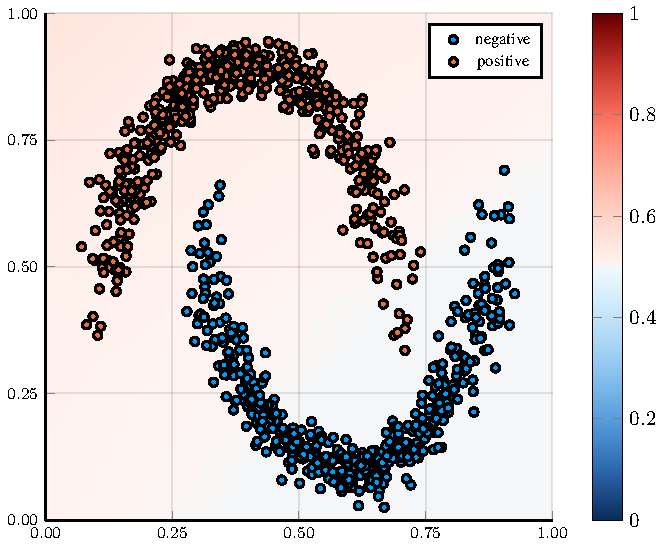
\includegraphics[width=0.6\pagewidth]{images/relu-heatmap/relu.pdf}
\end{frame}

\section{Závěr}

\begin{frame}{Závěr}
	\begin{itemize}
		\item Target propagation tak, jak byla implementována, není vhodnou alternativou ke zpětné propagaci.
		\item \cite{bartunov_assessing_2018} uvádí obdobné problémy na datasetu ImageNet.
		\item Další výzkum je třeba, zkoumající například:
		\begin{itemize}
			\item Vliv hyperparametrů
			\item Dynamické hodnoty hyperparametrů
			\item Regularizaci
		\end{itemize}
	\end{itemize}
\end{frame}

\begin{frame}{Seznam literatury}
	\printbibliography
\end{frame}

\end{document}
